\documentclass[12pt,a4paper]{article}
\usepackage[utf8]{inputenc}
\usepackage{graphicx}
\usepackage{amsmath}

\title{A Study on Bidirectional Document Conversion}
\author{Jane Doe}
\date{March 2026}

\begin{document}

\maketitle

\begin{abstract}
This paper presents a novel approach to bidirectional conversion between
LaTeX and Word document formats. We demonstrate that structural fidelity
can be maintained across round-trip conversions.
\end{abstract}

\section{Introduction}

Document format conversion is a common challenge in academic
collaboration. Many researchers prefer \textbf{LaTeX} for its
typesetting capabilities, while others use \textit{Microsoft Word}
for its accessibility.

% This is a comment that should survive round-trip
The challenge lies in preserving document structure across formats.

\section{Related Work}

Several tools exist for document conversion:

\begin{itemize}
  \item Pandoc provides general-purpose conversion
  \item LaTeX2RTF focuses on one-way conversion
  \item \textbf{Our approach} enables \underline{bidirectional} conversion
\end{itemize}

\subsection{Limitations of Existing Tools}

Current tools have significant limitations:

\begin{enumerate}
  \item Loss of formatting during conversion
  \item Poor handling of mathematical expressions
  \item No round-trip support
\end{enumerate}

\section{Methodology}

Our approach uses an intermediate representation (IR).
The conversion process follows these steps:

\begin{tabular}{| c | c | c |}
\hline
Step & Input & Output \\
\hline
1 & .tex file & IR tree \\
\hline
2 & IR tree & .docx file \\
\hline
3 & .docx file & IR tree \\
\hline
\end{tabular}

\subsection{Mathematical Expressions}

We support both inline math like $E = mc^2$ and display math:

\[
  \frac{\partial f}{\partial x} = \lim_{h \to 0} \frac{f(x+h) - f(x)}{h}
\]

\section{Results}

Our experiments show that the conversion maintains \textbf{95\%} structural
fidelity as measured by our IR comparison metric. See Figure~\ref{fig:results}
for details.

\begin{figure}[h]
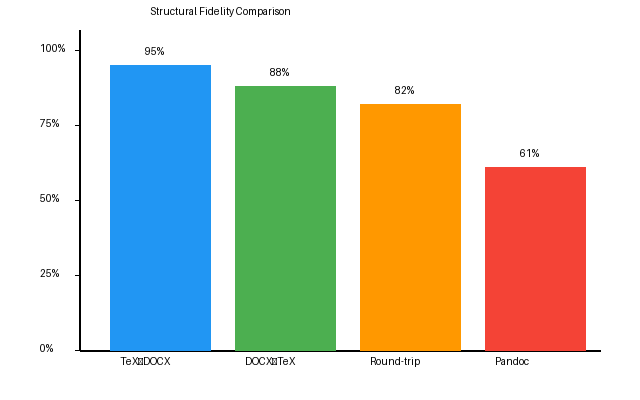
\includegraphics[width=0.8\textwidth]{images/figure1.png}
\label{fig:results}
\end{figure}

\section{Conclusion}

We have demonstrated a practical approach to bidirectional document
conversion. Future work will extend support to additional LaTeX
constructs and improve mathematical expression handling.

\cite{knuth1984texbook}
\cite{lamport1994latex}

\end{document}
